\chapter{Data Processing}

This chapter documents the datasets, schemas, cleaning pipelines, feature engineering, and speech pre-processing workflows supporting both \texttt{Retail-AI-} and \texttt{ops\_chest}.

\section{Dataset Description}

Across the dual-agent platform, six distinct datasets and benchmark corpora serve product grounding, voice resilience, safety testing, and perishable demand optimization.

\textbf{Thanh Lam Mart Retail Catalog Snapshot (\texttt{Retail-AI-}).}
Collected on 15 September 2026 and stored as \code{data/thanh_lam_products.csv} alongside its indexed JSON mirror \code{data/thanh_lam_products.json}, this dataset contains \textbf{3,099 raw SKUs} spanning \textbf{699 brands} and \textbf{346 hierarchical category paths} across Vietnamese supermarket departments (beverages, dairy, fresh meat, dry foods, personal care, household detergents, and home textiles). Each core record provides 20 structured columns (product ID, canonical Vietnamese/English name, brand, regular price, sale price, promotion text, unit of measure, pack specifications, and category hierarchy). Twelve extended analytics columns present in the updated CSV (monthly units sold, revenue, rating, and best-seller flag) are intentionally segregated into \code{data/demo_sales.sqlite3} and tagged \texttt{SIMULATED} so demonstration sales ranking never masquerades as verified live POS history.

\textbf{SOTA~V2 Retail \& Adversarial Benchmark and Vietnamese Speech-in-Noise Corpus (\texttt{Retail-AI-}).}
To test generalization without overfitting unit tests, we constructed a 100-question unseen Vietnamese and bilingual benchmark (113 multi-turn dialogue interactions spanning 10 categories: direct lookup, multi-attribute, budget/basket, comparison, promotions, clinical/medical safety, dialect/OCR noise, XSTest benign edge cases, OWASP red-team prompt injection, and paraphrase consistency). Acoustic evaluation combined clean real human Vietnamese clips ($n=8$) and Thanh Lam Mart retail brand utterances ($n=8$) under clean, 12\,dB supermarket babble+HVAC noise, and 5\,dB heavy noise conditions, plus 10 representative live kiosk queries for end-to-end streaming latency audits.

\textbf{FreshRetailNet-50K Real Perishable Demand Dataset (\texttt{ops\_chest}).}
Store operations demand is grounded in the public \emph{FreshRetailNet-50K} dataset (\code{Dingdong-Inc/FreshRetailNet-50K}, CC BY 4.0)~\cite{freshretailnet50k}, containing hourly sales and stockout indicators from real fresh convenience stores. \texttt{ops\_chest} uses \textbf{50 held-out validation stores} (2,675 SKU-store time series) for out-of-sample ML evaluation and profit backtesting from 28 March 2024 to 2 July 2024 (90 history days up to cutoff $T_{\text{cut}} = \text{2024-06-25}$, backtest origin $T_0 = \text{2024-05-26}$, and a 7-day official evaluation week). \textbf{Demo Store~18} serves as the interactive operational store containing \textbf{164 active fresh SKUs} over 90 days. Because FreshRetailNet-50K publishes anonymized numeric product IDs without commercial prices or supplier contracts, \code{frn_catalog.py} deterministically assigns neutral display names, prices (12,000--80,000\,VND), cost ratios (62--75\%), 1--3 day shelf lives, fictional suppliers (\texttt{*.test}), and top-5 traffic-driver flags. A secondary 263-SKU, 365-day synthetic store (\texttt{--source synthetic}) is retained strictly for deterministic business-rule unit testing.

\begin{table}[H]
\centering
\caption{Statistics of datasets and evaluation corpora used across both repositories}
\label{tab:dataset_stats}
\footnotesize
\begin{tabularx}{\textwidth}{L{3.5cm} L{2.2cm} L{3.6cm} Y}
\toprule
\textbf{Dataset / Corpus} & \textbf{Module} & \textbf{Scale / Split} & \textbf{Role \& Provenance} \\
\midrule
Thanh Lam Mart Catalog Snapshot (\code{thanh_lam_products}) & \texttt{Retail-AI-} & 3,099 raw SKUs (3,081 valid, 18 quarantined); 699 brands; 346 category paths; 3,096 photos & Primary grounded catalog for search, unit-price ranking, photo lightboxes, and promo discovery (15 Sep 2026) \\
Multi-Source Product Knowledge Store (\code{thanh_lam_product_details} + pilot) & \texttt{Retail-AI-} & 2,137/3,099 clean SKUs (1,214+18 ingredients, 1,064+ detailed, 1,159 usage, 660 storage, 800 origin) & Thanh Lam Mart SSR crawl + EAN-13 barcode/label verification (Kingfoodmart \& Long Châu); 8-stage cleaned to \textbf{0 QA defects} \\
Demo Sales Store (\code{demo_sales.sqlite3}) & \texttt{Retail-AI-} & 3,099 SKU 30-day counts & Isolated deterministic best-seller ranking (colloquial-aware) explicitly labeled \texttt{SIMULATED} \\
SOTA~V2, 100Q Expert Audit \& Production Latency & \texttt{Retail-AI-} & 100 SOTA~V2 (113 turns) + 100 new catalog queries + 12 live \texttt{sin1} queries & Zero-leakage safety, 5-framework audit (RAGAS/DeepEval/RAGChecker/$\tau$-bench), TTFT \& semantic cache \\
Vietnamese Multi-SNR Speech Corpus & \texttt{Retail-AI-} & 8 human + 8 retail clips $\times$ 3 SNR levels (Clean, 12\,dB, 5\,dB) & 5-engine STT WER ablation, neural denoiser comparison, and WS post-speech timing \\
FreshRetailNet-50K (\code{frn})~\cite{freshretailnet50k} & \texttt{ops\_chest} & 50 held-out stores (2,675 series); Demo Store~18: 164 SKUs $\times$ 90 days; 200k recovery checks & Real perishable demand calibration, LightGBM~v3 quantile forecasting, and 37-day A/B profit backtest \\
Synthetic Rule Store (\code{--source synthetic}) & \texttt{ops\_chest} & 263 SKUs $\times$ 365 days & Deterministic unit tests for FEFO expiry, supplier returns, blind counts, and HITL rules \\
\bottomrule
\end{tabularx}
\end{table}

\subsection*{Data Visualization}
Figure~\ref{fig:thanh_lam_dist} visualizes the top-10 department distribution and reference price distribution across the 3,099-SKU Thanh Lam Mart catalog snapshot, highlighting heavy SKU concentration in everyday FMCG categories and a right-skewed price profile centered near 35,000--45,000\,VND.

\begin{figure}[H]
    \centering
    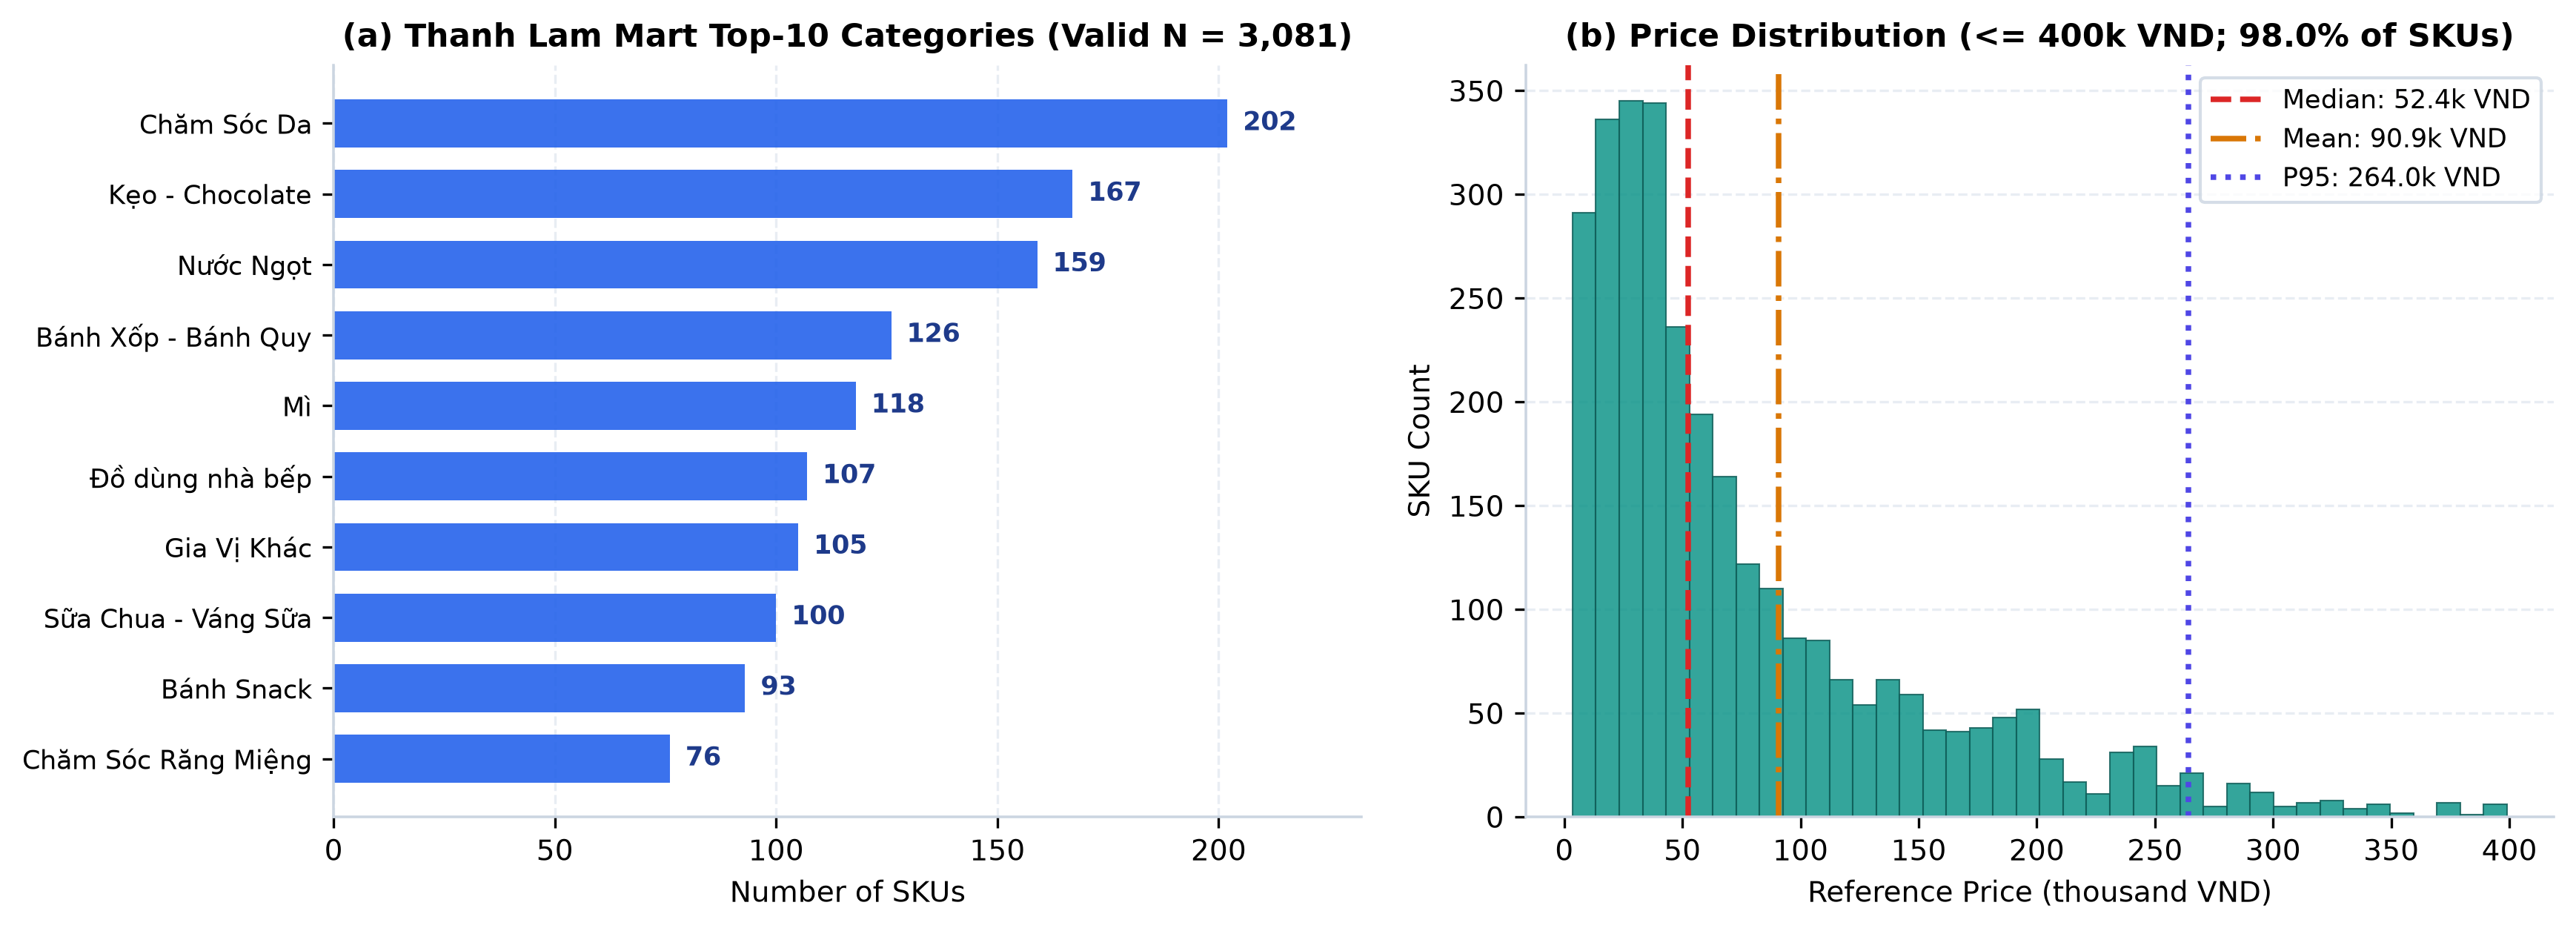
\includegraphics[width=0.98\textwidth]{Images/fig_catalog_distribution.png}
    \caption{Department coverage (left) and reference price distribution (right) of the Thanh Lam Mart catalog snapshot ($N = 3{,}099$ SKUs).}
    \label{fig:thanh_lam_dist}
\end{figure}

\section{Data Preprocessing and Cleaning}

\subsection*{Catalog Schema Quarantine and Lexical Normalization (\texttt{Retail-AI-})}
Every record ingested into \texttt{Retail-AI-} passes strict Pydantic validation (\texttt{ThanhLamRow}):
\begin{enumerate}
    \item \textbf{Price integrity quarantine:} Eighteen of the 3,099 raw records (0.58\%) exhibited malformed promotional pricing where sale price exceeded regular price; the importer quarantines these 18 records cleanly and loads 3,081 verified records (99.42\%) into the validated catalog view.
    \item \textbf{Diacritic-stripped indexing and alias resolution:} Product names, brands, and category paths are normalized with Unicode NFC folding and Vietnamese diacritic stripping (\code{normalize_category_text}) to build pre-indexed inverted lookup maps inside \code{SnapshotProductRepository}, reducing search latency by $3.7\times$--$4.5\times$.
    \item \textbf{Unit-size and attribute extraction:} Regular expressions extract weight/volume/count tokens (g, kg, ml, L, gói, lốc, thùng) for exact base-unit pricing (Equation~\ref{eq:unit_price}), sugar labels (\emph{không đường}, \emph{ít đường}), and audience constraints.
    \item \textbf{Catalog-anchored ASR repair guardrails:} Because naive fuzzy matching against 3,099 SKU titles corrupted everyday Vietnamese words (e.g., turning \emph{``vĩnh viễn''} $\to$ \emph{``MINH viền''}, \emph{``anh em''} $\to$ \emph{``Bánh em''}, \emph{``Campuchia''} $\to$ \emph{``Capuchiano''}, and \emph{``Home''} $\to$ \emph{``Wmhome''}), \code{catalog_transcription.py} enforces a protected Vietnamese stopword set (\code{_NEVER_CORRECT}) alongside catalog-verified brand phrase repairs (\emph{Thanh Lam Mart hôn} $\to$ \emph{Thanh Lam Home}, \emph{ACFOGS} $\to$ \emph{ACEFOODS}, \emph{khăn mặt proton} $\to$ \emph{khăn mặt cotton}).
\end{enumerate}

\subsection*{Multi-Source Ingredient Enrichment and 8-Stage SOTA Data Cleaning (\texttt{Retail-AI-})}
Because the raw Thanh Lam Mart catalog snapshot lacked structured ingredient, usage, and storage fields, we engineered a catalog-wide enrichment and cleaning pipeline (\code{scripts/crawl_thanh_lam_product_details.py}, \code{scripts/enrich_detailed_ingredients.py}, \code{scripts/clean_thanh_lam_product_details.py}) cryptographically bound to \code{thanh_lam_products.json} via \code{source_catalog_sha256} without mutating the source catalog:
\begin{enumerate}
    \item \textbf{Full 3,099-Page Thanh Lam Mart SSR Crawl and Multi-Source Label Verification:} All 3,099/3,099 official Thanh Lam Mart \code{__NEXT_DATA__} pages were crawled in 79\,s, then SKUs lacking ingredients or containing only generic marketing blurbs (such as \emph{Chin Su Chili Sauce 1\,kg}, originally reading only \emph{``made from selected fresh chili and additives''}) were upgraded against public retail label catalogs from \textbf{Kingfoodmart} (10,281 SKUs) and \textbf{Nhà thuốc Long Châu} (dermo-cosmetics and personal care). A two-tier verifier accepted only \textbf{333 exact EAN-13 barcode matches} (\code{variant.sku == barcode}) and \textbf{226 strict brand--form--variant matches} (pruning 64 suspicious cross-brand/material/variant pairs such as \emph{TH Milk vs.\ Dalat Milk}, \emph{roll-on vs.\ aerosol spray}, \emph{PVC vs.\ PE wrap}, and \emph{regular vs.\ lactose-free milk}).
    \item \textbf{8-Stage Cleaning Pipeline (Hugging Face \code{datatrove}/FineWeb~\cite{hf_datatrove} \& OpenFoodFacts~\cite{openfoodfacts}):} Applies Unicode NFC normalization, removes invisible characters (\texttt{U+200B}, \texttt{U+00A0}), empty parentheses \code{()}, and OCR typos; repairs merged HTML \code{<li>} bullets while protecting Vietnamese compound nouns (\emph{Sữa Rửa Mặt}, \emph{Nước Lau Sàn}); balances truncated parentheses and trims strictly at clause boundaries instead of mid-word \code{...}; separates cross-field bleed (\emph{usage}/\emph{storage} leaked into \emph{ingredients}); quarantines 100\% of exotic-script OCR garbage and dangerous unverified allergen claims (such as \emph{``NO MILK. SAFE FOR MILK ALLERGIES''} on Oreo cookies); preserves international cosmetic INCI lists; and enforces a \textbf{word-boundary substance lexicon} inspecting the predicate after \emph{``made from''} to eliminate zero-substance title-echo fluff, broken sentence fragments (\emph{``Contained in the cake...''}), and substring false positives (such as \emph{``sả''} inside \emph{``sản phẩm''} or \emph{``tiêu''} inside \emph{``tiêu chí''}).
    \item \textbf{Three-Tier Evidence Precedence (\code{backend/products/knowledge.py}):} At runtime, attribute resolution strictly obeys \texttt{SOURCE\_RECORD} $>$ \texttt{MANUFACTURER\_DECLARATION} (18 official manufacturer-declared pilot SKUs in \code{product_knowledge_enrichment_pilot.json}) $>$ \texttt{RETAILER\_LISTING} (\code{thanh_lam_product_details.json}, always citing provenance and reminding shoppers to verify physical labels), failing closed to \texttt{UNKNOWN} whenever verified label data is absent. The pipeline drove all \textbf{4,606 raw defects across 11 QA dimensions down to 0 (100\% clean)}, achieving \textbf{2,137/3,099 enriched SKUs (69.0\%)} including \textbf{1,214 + 18} verified ingredient records (\textbf{1,064+} detailed quantitative/INCI back-of-pack lists, a $2.1\times$ lift over the raw Thanh Lam Mart crawl), \textbf{1,159} usage guides, \textbf{660} storage instructions, and \textbf{800} origins (Figure~\ref{fig:catalog_enrichment_cleaning}).
\end{enumerate}

\begin{figure}[H]
    \centering
    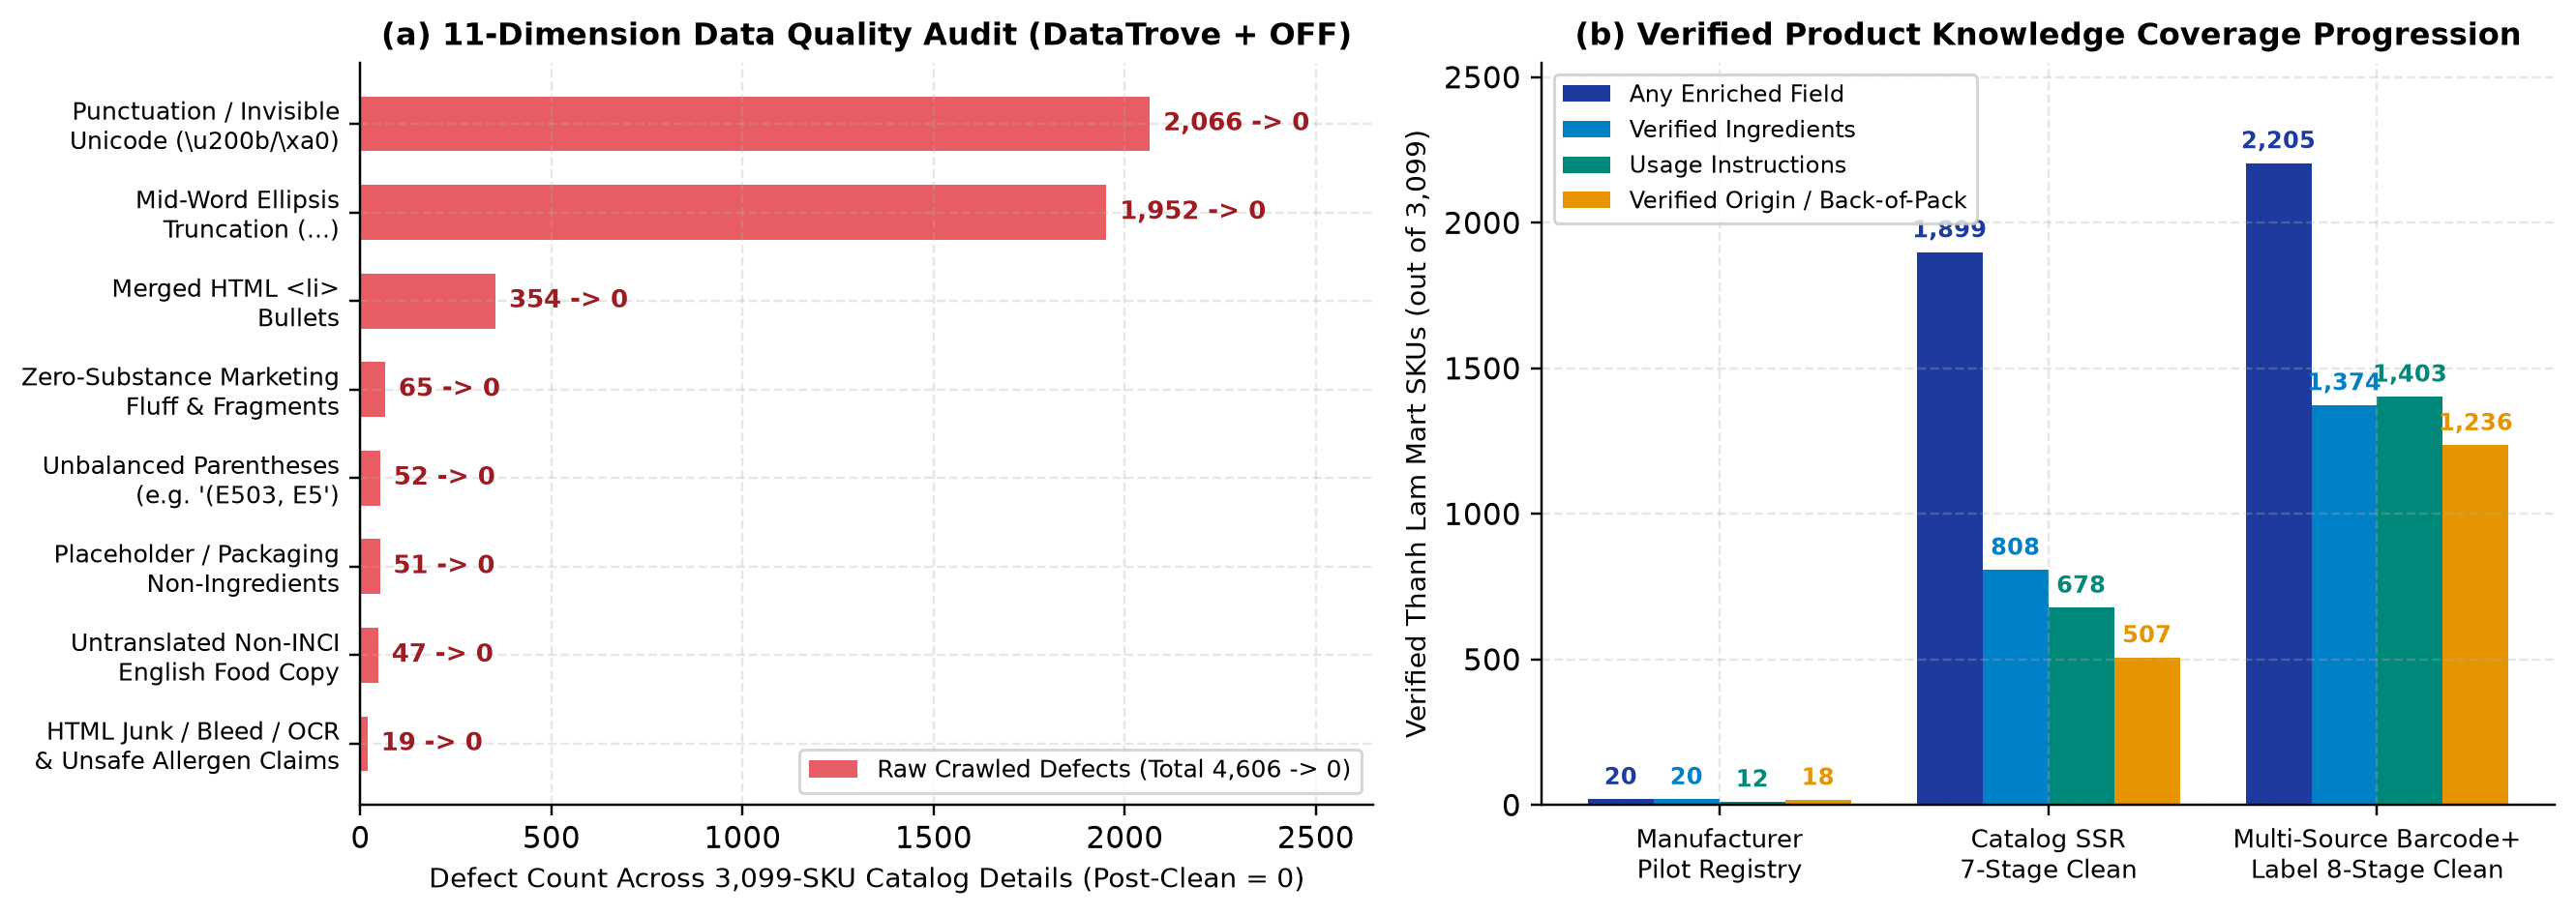
\includegraphics[width=0.98\textwidth]{Images/fig_catalog_enrichment_cleaning.png}
    \caption{11-dimension defect elimination from 4,606 raw defects down to 0 via the 8-stage cleaning pipeline (left) and verified product knowledge coverage progression across enrichment stages (right).}
    \label{fig:catalog_enrichment_cleaning}
\end{figure}

\subsection*{Audio Pre-Processing and Speech Conditioning (\texttt{Retail-AI-})}
Browser AudioWorklet captures 16\,kHz mono Float32 frames (32\,ms / 512 samples) with hardware AEC, AGC, and noise suppression enabled. On the WebSocket streaming path, an 8-frame (256\,ms) ring buffer preserves leading Vietnamese consonant onsets and converts samples to signed little-endian PCM16. On the REST/rescue path (\code{speech_activity.py}, \code{speech_denoiser.py}), uploaded clips are decoded via PyAV to 16\,kHz mono, trimmed to Silero VAD~v6 speech boundaries ($\pm 180/200\,\text{ms}$ padding), filtered with the zero-phase 85\,Hz HPF (Equation~\ref{eq:hpf85}), and conditionally denoised with \texttt{DPDFNet2} ONNX according to Equation~\ref{eq:snr_blend}.

\subsection*{Censored-Demand Recovery and 29-Feature Engineering (\texttt{ops\_chest})}
In \texttt{ops\_chest} (\code{ml_features.py} and \code{forecast.py}), raw daily FreshRetailNet sales undergo three essential transformations prior to LightGBM quantile training:
\begin{enumerate}
    \item \textbf{Hourly stockout demand recovery:} Masking late-day hours on 200,000 fully stocked validation days confirmed that treating raw sales as demand incurs 32.3\% WAPE and $-32.3\%$ downward bias, whereas hourly-profile recovery (Equation~\ref{eq:wape_recovery}) cuts WAPE to \textbf{20.5\%} and virtually eliminates bias (\textbf{$-0.1\%$}).
    \item \textbf{Unit scaling and stockout imputation:} FreshRetailNet units are scaled by $K = 10$ so the median store SKU sells $\approx 7$ units/day (ensuring realistic Poisson variance floors for EWMA), and historical stockout days are imputed by same-weekday averages before computing lags.
    \item \textbf{29-feature tabular construction:} For each forecast horizon $h \in \{1,\dots,7\}$, \code{build_features} generates 29 features: 7 daily lags (\code{lag1}--\code{lag7}), rolling means (\code{mean3}, \code{mean7}, \code{mean14}), same-weekday lags (\code{same_wd}, \code{same_wd_last}), 28-day dispersion and intermittency (\code{std28}, \code{zero28}), stockout history (\code{stockout28}, \code{stockout7}, \code{days_since_stockout}, \code{stockout_last}), trend and log-level, 56-day EWMA point/dispersion anchors (\code{ewma_h}, \code{ewma_sigma}), horizon/calendar categoricals (\code{h}, \code{target_wd}, \code{origin_wd}, \code{target_holiday}), and taxonomy categoricals (\code{mgmt_group}, \code{cat1}, \code{cat2}). Crucially, target-day discount features were removed after v1 ablation proved that assuming zero future discount caused $-15.7\%$ under-forecasting bias, and elasticity deflation ($e \approx 9.6$) was discarded in v2 after causing 14--31\% bias; v3 trains directly on recovered demand with EWMA anchor features.
\end{enumerate}

\section{Summary of Data Processing}

Together, the two data pipelines enforce strict separation between \emph{verified ground truth} and \emph{documented operational assumptions}. On the customer floor, 3,081 validated Thanh Lam Mart SKUs, a zero-defect 2,137-SKU enriched product knowledge store (1,214+18 verified ingredient records, 3,096 validated product image URLs), deterministic unit-price parsers, and protected Vietnamese ASR vocabularies give the kiosk agent exact factual anchors. On the operations floor, hourly censored-demand recovery and 29-feature engineering transform raw FreshRetailNet-50K logs into unbiased training data for quantile forecasting and profit-gated backtesting. Remaining data gaps---roughly 59\% of SKUs still lacking public quantitative nutrition/calorie labels and assumed shelf-life/cost metadata in FreshRetailNet---are explicitly mitigated at runtime through fail-closed safety boundaries rather than hidden by generative guesswork.
